\usetikzlibrary{patterns}
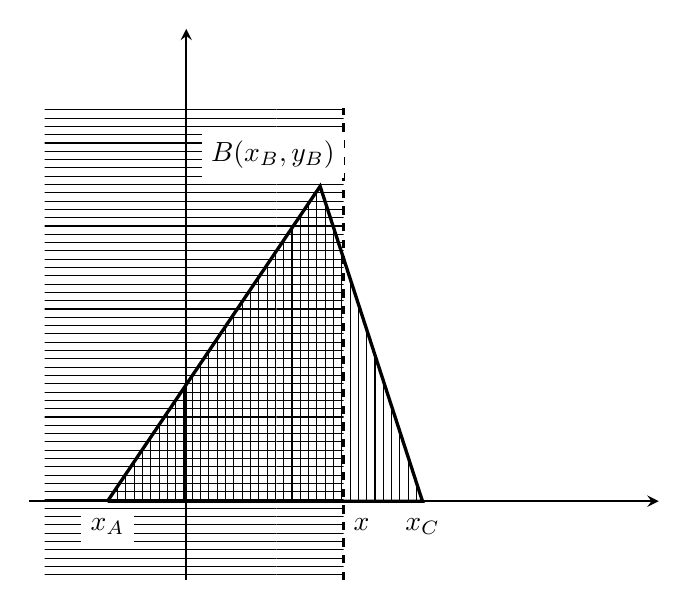
\begin{tikzpicture}

\draw[thick,-stealth]  (0,-1) -- (0,6);
\draw[thick,-stealth] (-2,0) -- (6,0);
\draw[very thick, pattern=vertical lines] (-1,0) -- (1.7, 4) -- (3,0) -- (-1, 0);
\draw[very thick, dashed] (2, -1) -- (2, 5);
\path[pattern=horizontal lines] (2, -1) rectangle (-1.8, 5);

\node[below, fill = white] at (-1,-0.1) {$x_A$};
\node[above, fill = white] at (1.1,4.1) {$B(x_B, y_B)$};
\node[below] at (3,-0.1) {$x_C$};
\node[below right] at (2,-0.1) {$x$};

\end{tikzpicture}